\section{Billboards}
\label{sec:vis_billboards}
We could in principle create a spherical shape by connecting triangles or other primitives as illustrated in figure \ref{fig:visualization_glut_spheres}. The figure contains two spheres with different numbers of primitives. We need a substantial number of primitives to get a shape that looks like a sphere (200 in the left sphere in the figure), but we can cheat a bit, by instead rendering something that \textit{looks} like a sphere
\begin{figure}[h]
\begin{center}
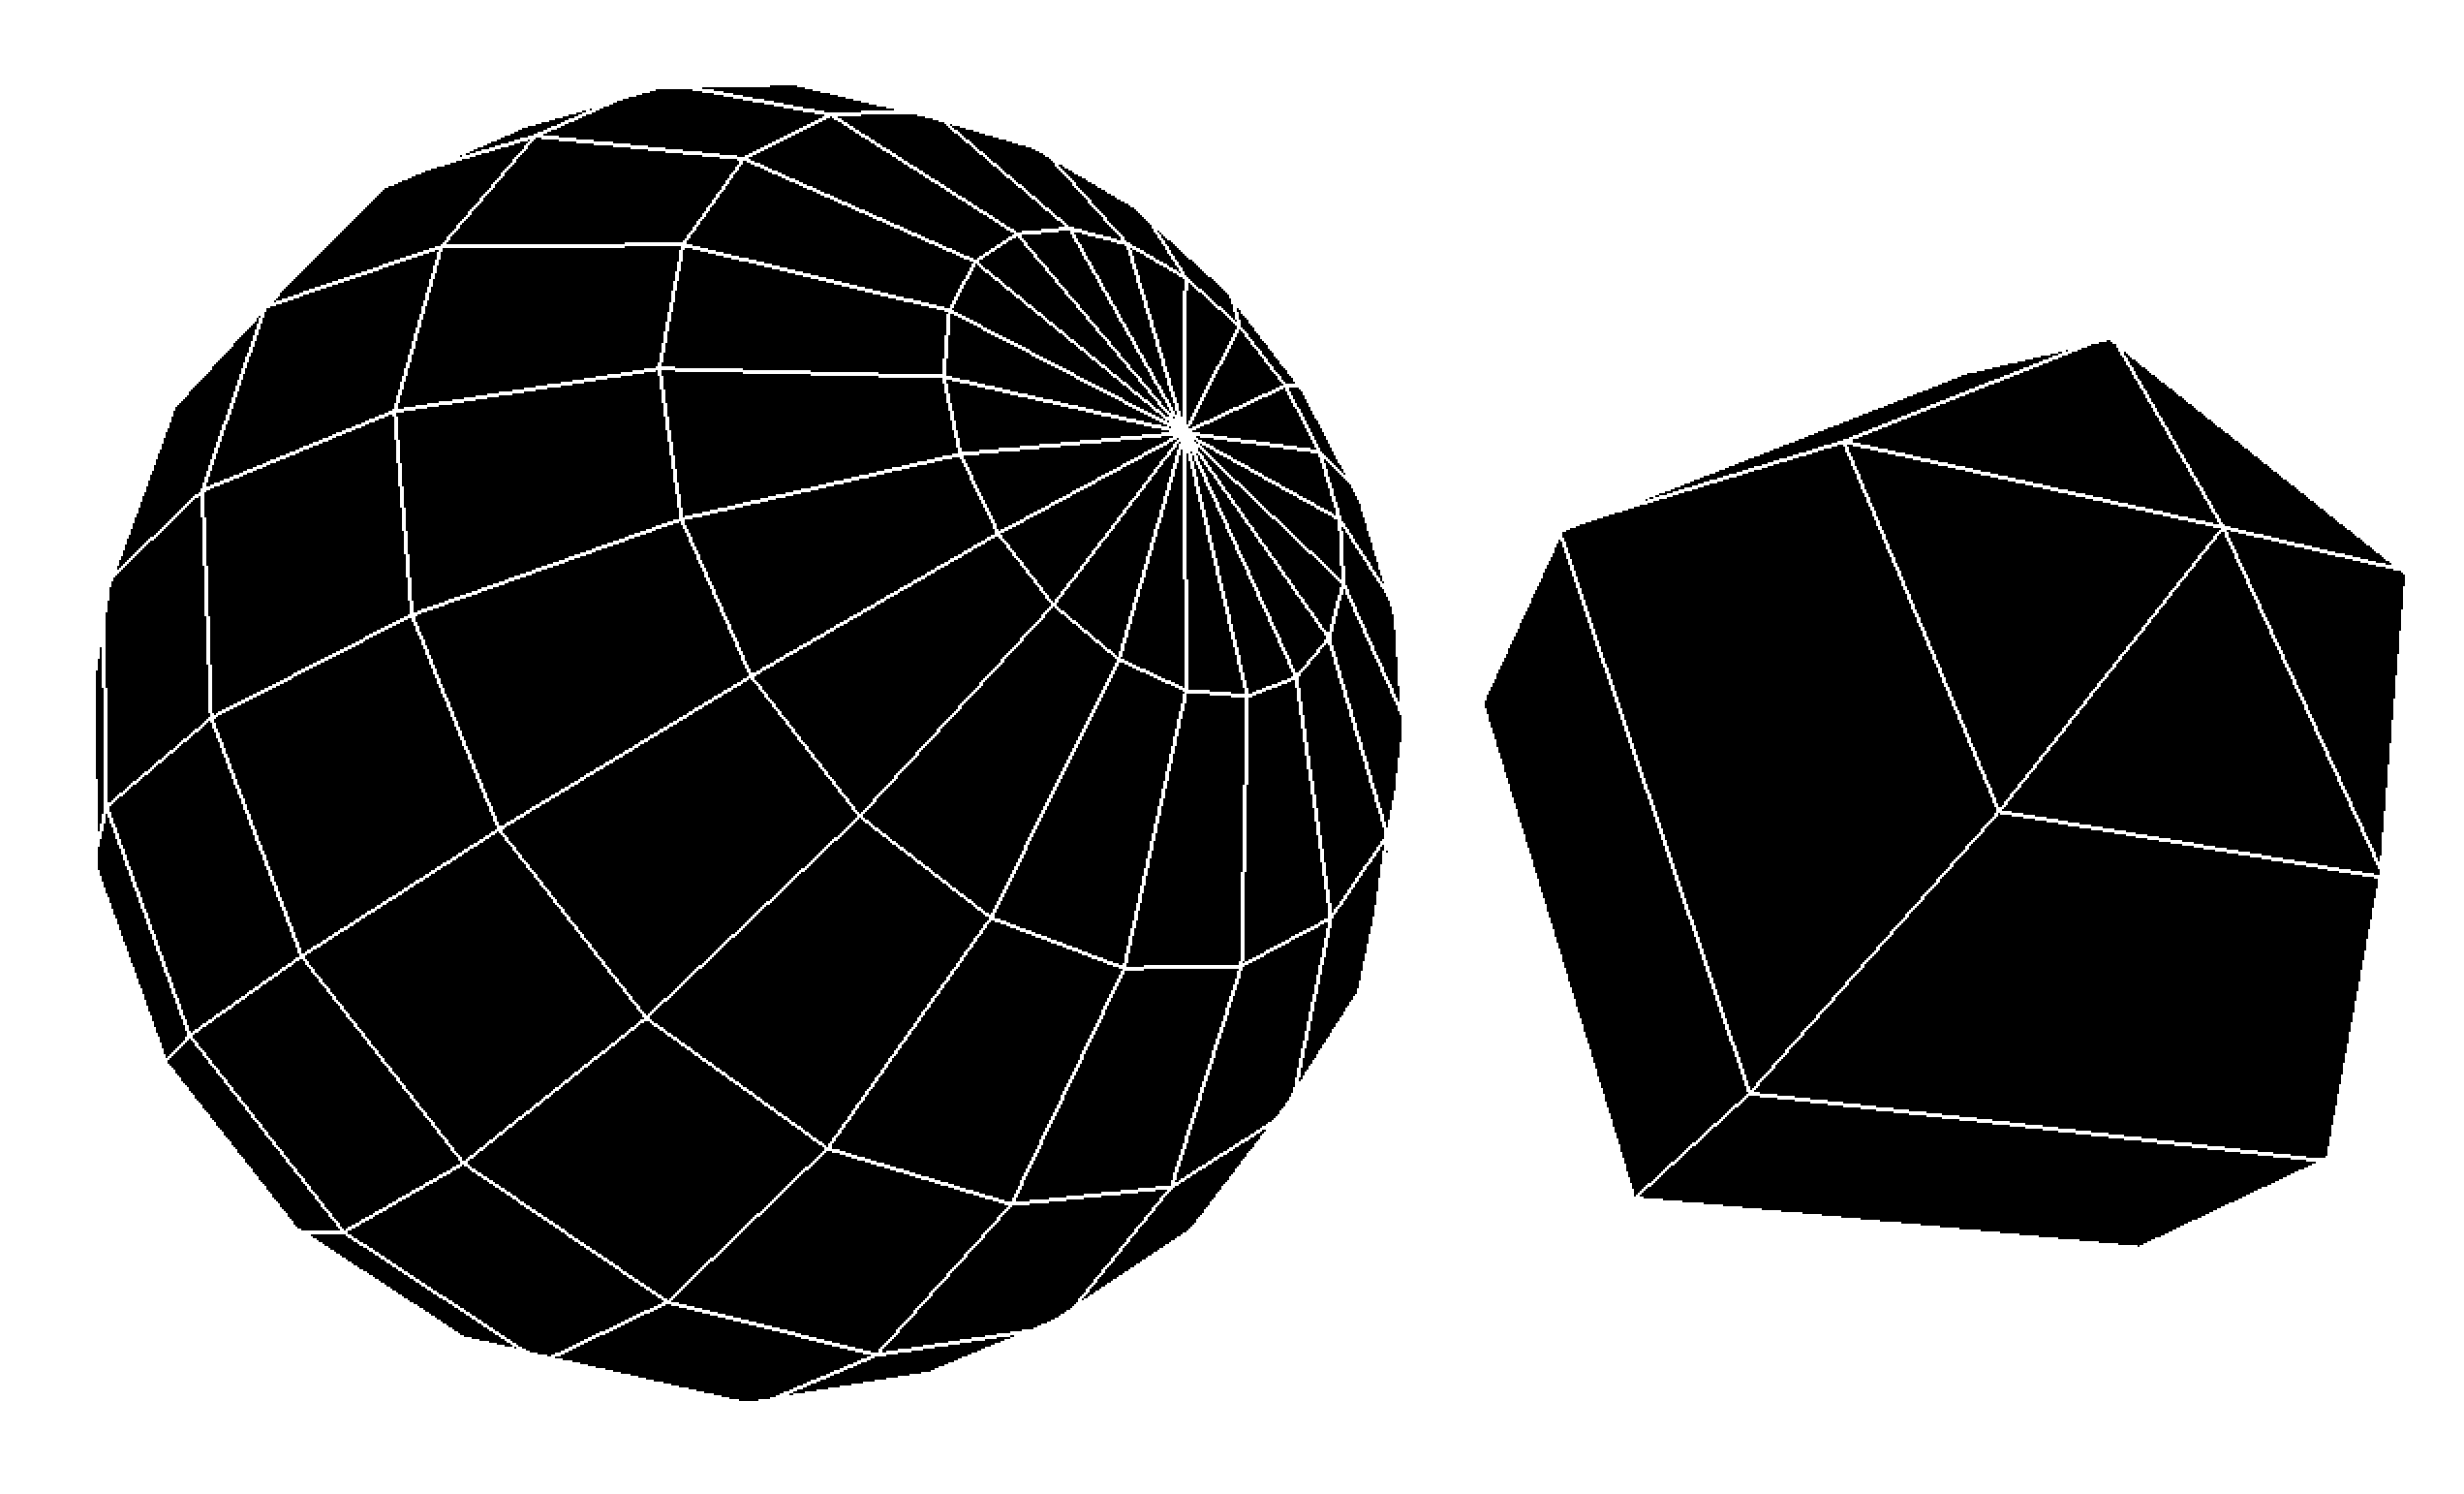
\includegraphics[width=0.8\textwidth, trim=0cm 0cm 0cm 0cm, clip]{visualization/figures/glut_spheres.png}
\end{center}
\caption{A sphere can be created by connecting triangles or other primitives. The sphere to the left is made of 200 primitives whereas the one to the right is made of 25 primitives. It is clear that we need a certain number, more than 25, of primitives before we are convinced that the object should represent a sphere.}
\label{fig:visualization_glut_spheres}
\end{figure}
A billboard is, as the name suggests, a rectangle filled with a texture, always pointing towards the camera. The texture is going to be a circle (a sphere does indeed look like a circle when rendered on the screen anyway). It is quite easy to render such a rectangle with OpenGL, we already have a primitive called \textit{GL\_QUADS} which is exactly what we need. The only thing we need to do is provide four vertices, the corners in the rectangle, and give each vertex a texture coordinate. The four vertices $\vec v_i$ can be calculated from one single vertex $\vec r$, the particle position, by
\begin{align}
	\label{eq:vis_vertices_billboard}
	\vec v_1 &= \vec r + (-\Delta x, -\Delta y)\\
	\nonumber
	\vec v_2 &= \vec r + (-\Delta x, \Delta y)\\
	\nonumber
	\vec v_3 &= \vec r + (\Delta x, \Delta y)\\
	\nonumber
	\vec v_4 &= \vec r + (\Delta x, -\Delta y),
\end{align}
where ($L_x = 2\Delta x, L_y = 2\Delta y$) is the size of the billboard, see figure \ref{fig:visualization_billboard_vertices}.
\begin{figure}[h]
\begin{center}
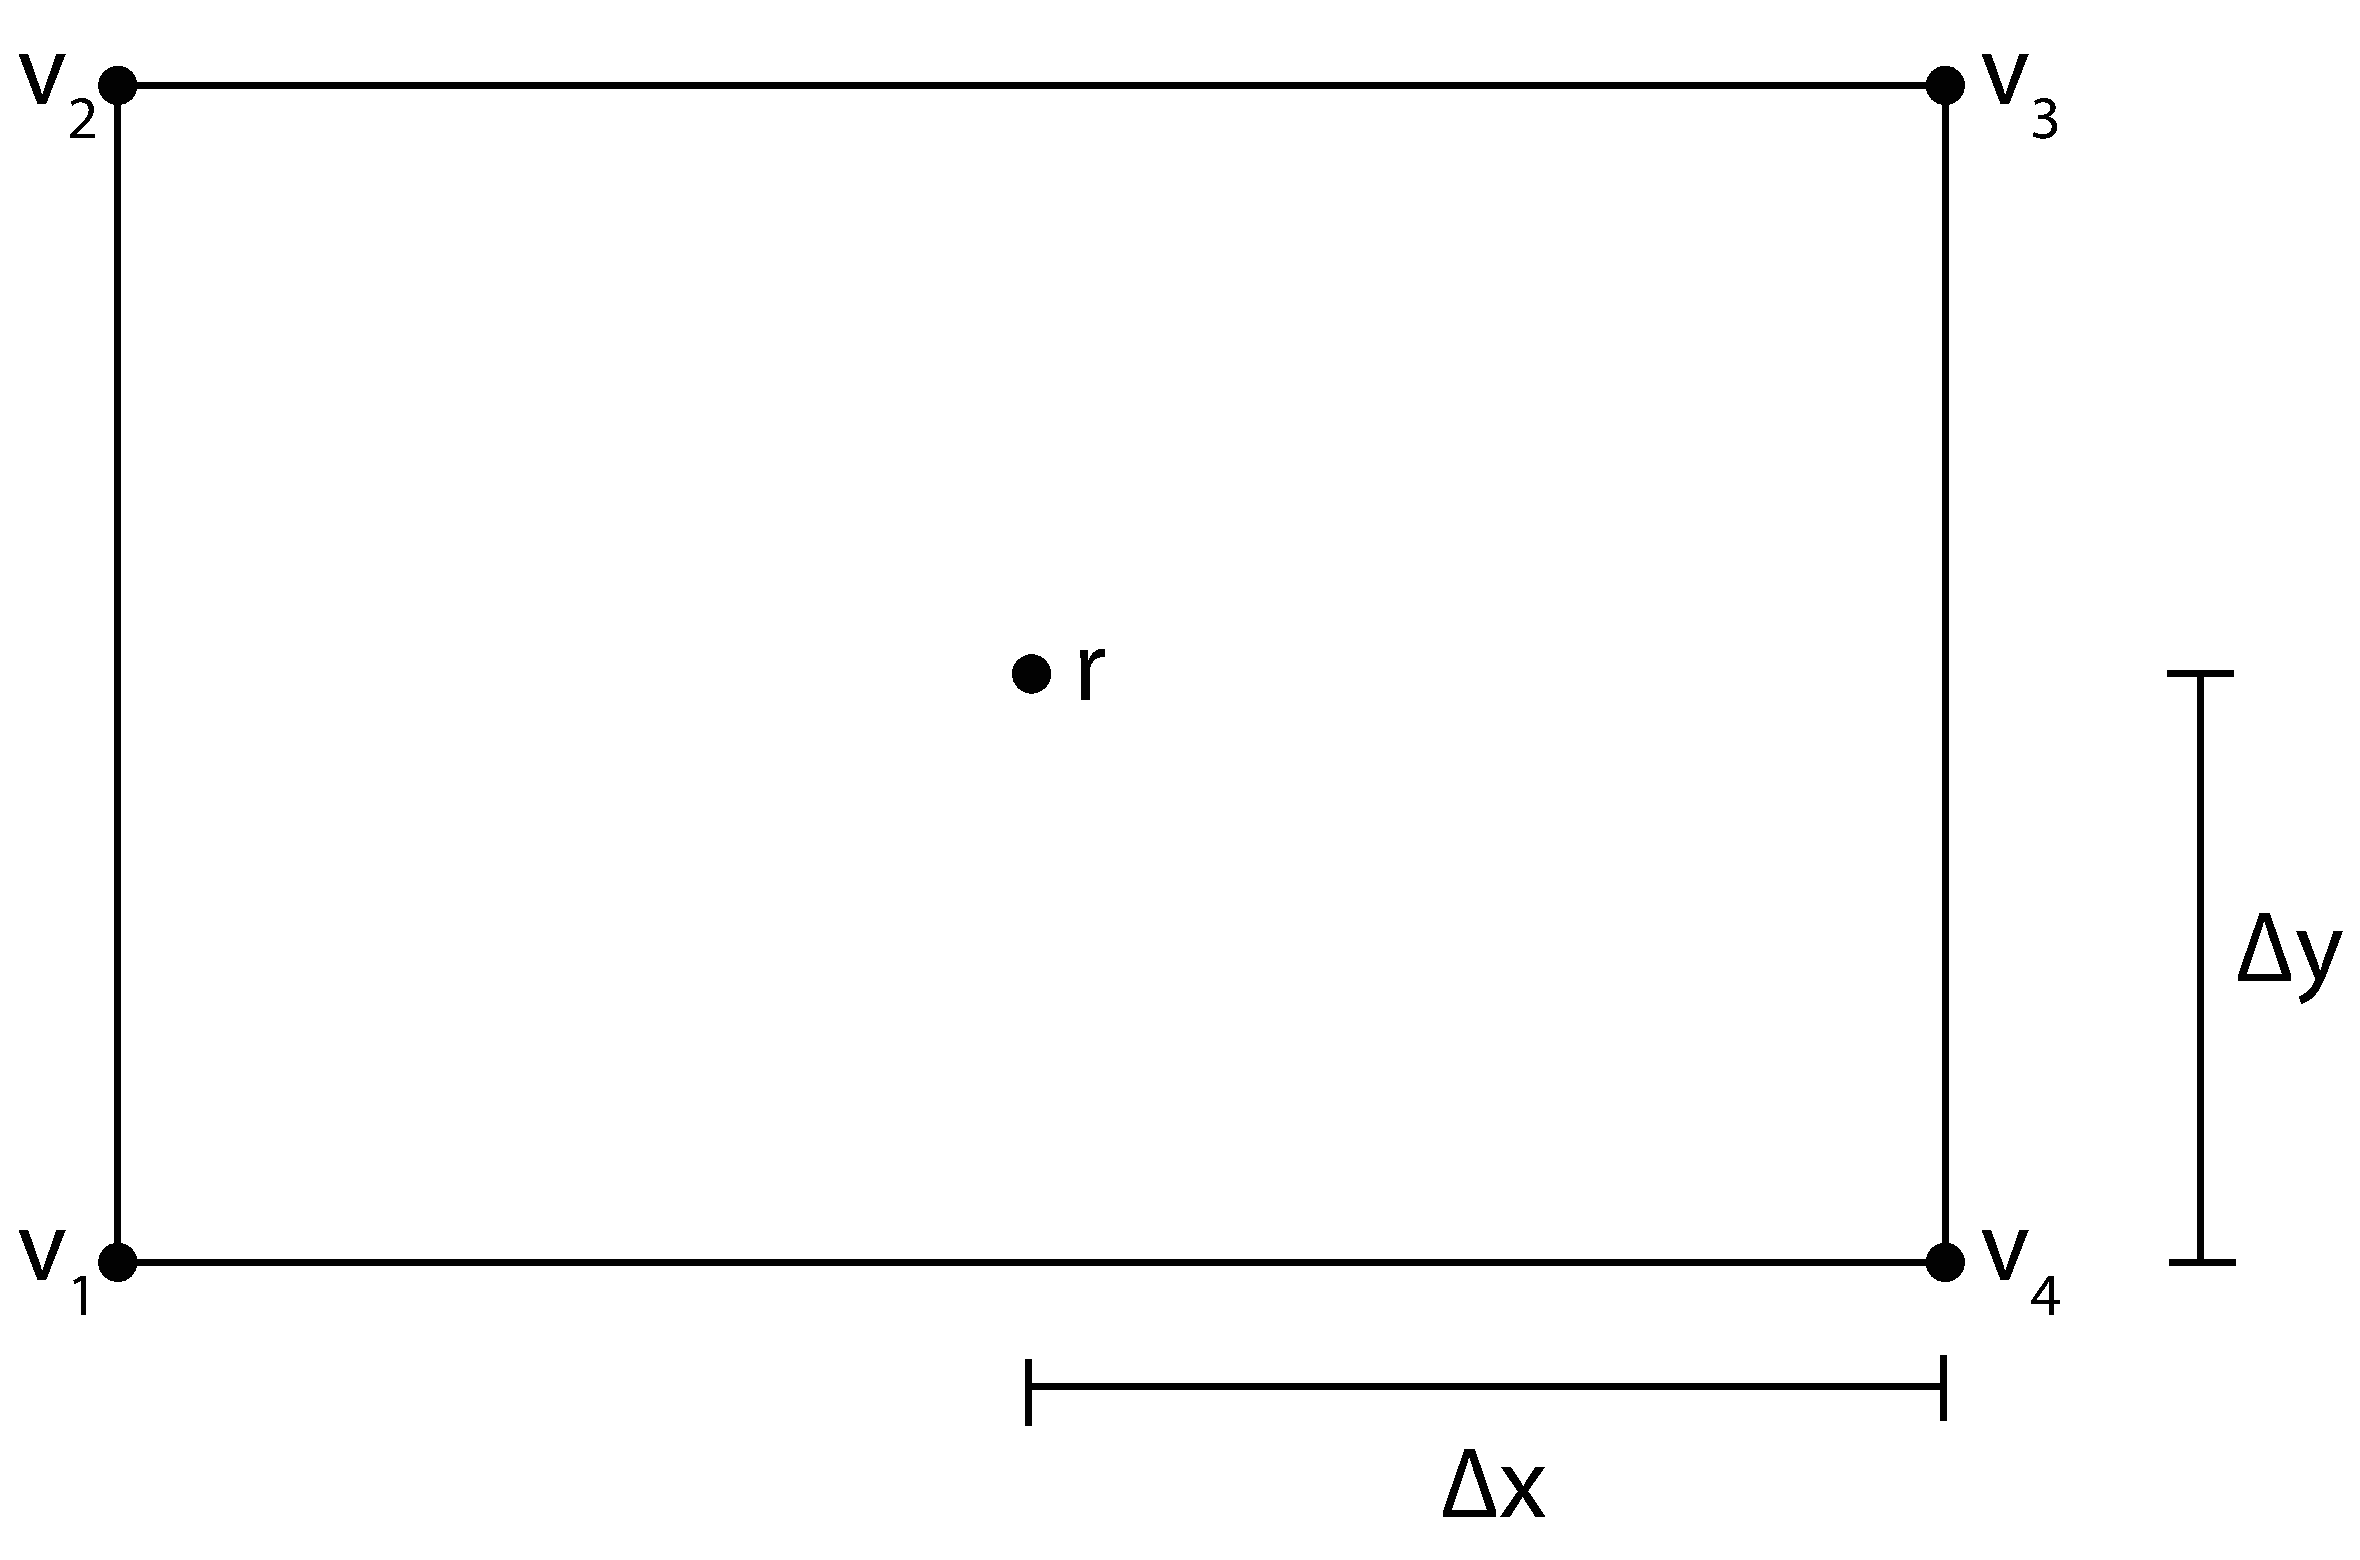
\includegraphics[width=0.7\textwidth, trim=0cm 0cm 0cm 0cm, clip]{visualization/figures/billboard.eps}
\end{center}
\caption{A billboard is made of four vertices $\vec v_1, \vec v_2, \vec v_3$ and $\vec v_4$ that can be calculated from one vertex $\vec r$ (equation \eqref{eq:vis_vertices_billboard}).}
\label{fig:visualization_billboard_vertices}
\end{figure}
This is already what Ovito does\footnote{See the source code at \url{http://www.ovito.org/index.php/download2}}, but we are going to improve this even more. Instead of computing the four vertices and uploading these as \textit{GL\_QUADS} to the GPU, we will only upload the positions of the particles, and exploit the geometry shader to create the billboard vertices on the GPU.

Before we start visualizing the data, all timesteps of a simulation are uploaded as VBO's on the GPU so that we don't need to upload data every frame. The VBO is rendered as \textit{GL\_POINTS} so each vertex represents the center position of a particle. We will now follow a single vertex through the pipeline
\subsection{The pipeline}
The VBO can now be seen as one OpenGL model containing the positions of all the particles. The vertices are then in the \textit{model space}. Every single vertex starts its life in the pipeline by going into the vertex shader. The vertex shader is pretty simple in this case, it just transforms the input vertex from the model space to the projection space as we can see in listing \ref{lst:simplevertexshaderbillboard}.
\begin{lstlisting}[caption=billboardVertexShader.glsl, label=lst:simplevertexshaderbillboard, language=GLSL]
#version 330\n"
uniform mat4 qt_ModelViewProjectionMatrix;
in vec4 qt_Vertex;
void main(void)
{
    gl_Position = qt_ModelViewProjectionMatrix * qt_Vertex;
}
\end{lstlisting}
This position is then sent to the geometry shader as an instance of the \textit{GL\_POINTS} primitive. The geometry shader will, from that single vertex (the position, now in the projection space), create and emit \textit{four} vertices that are displaced from the input vertex as explained in equation \eqref{eq:vis_vertices_billboard} and figure \ref{fig:visualization_billboard_vertices}. The output primitive is here the \textit{GL\_TRIANGLE\_STRIP} which will create two triangles with vertices $\{\vec v_1, \vec v_2, \vec v_3\}$ and $\{\vec v_2, \vec v_3, \vec v_4\}$. The size of the billboard is available as a uniform (as explained in subsection \ref{sec:opengl_uniforms}) in the geometry shader. If we want to visualize particles with different sizes (e.g. two atom types with different atomic radii), we just render different VBO's with the corresponding size. We want the four vertices to form a rectangle pointing towards the camera, so the operation in equation \eqref{eq:vis_vertices_billboard} should be done in the view space (here the $z$-direction is orthogonal on the camera plane which forms the $xy$-plane). Since the position vertex now is in the projection space, we should transform the four displacement vectors to the projection space by applying the \textit{qt\_ProjectionMatrix} before we add them together. We then set the texture coordinate (the local coordinate in the texture image) on each vertex and emit it with the \textit{EmitVertex()} function. The algorithm might be easier to understand with a code example, see listing \ref{lst:simplegeometryshaderbillboard}.

\begin{lstlisting}[caption=billboardGeometryShader.glsl, label=lst:simplegeometryshaderbillboard, language=GLSL]
#version 400
layout( points ) in;
layout( triangle_strip, max_vertices = 4 ) out;
uniform mat4 qt_ProjectionMatrix;
uniform vec2 size;
out vec2 texCoord;

void main(void) {
    vec4 pos = gl_in[0].gl_Position;
    gl_Position = pos + qt_ProjectionMatrix*vec4(-size.x, -size.y, 0.0, 0.0);
    texCoord = vec2(0.0, 0.0);
    EmitVertex();
    gl_Position = pos + qt_ProjectionMatrix*vec4(-size.x, size.y, 0.0, 0.0);
    texCoord = vec2(0.0, 1.0);
    EmitVertex();
    gl_Position = pos + qt_ProjectionMatrix*vec4(size.x, -size.y, 0.0, 0.0);
    texCoord = vec2(1.0, 0.0);
    EmitVertex();
    gl_Position = pos + qt_ProjectionMatrix*vec4(size.x, size.y, 0.0, 0.0);
    texCoord = vec2(1.0, 1.0);
    EmitVertex();
    EndPrimitive();
}
\end{lstlisting}
This is done with every single position vertex in the VBO (once per particle per frame) and all the output primitives from the geometry shader will be rasterized, clipped and texture coordinates are interpolated into the fragment shader that is run once per pixel per visible primitive. Before we discuss the fragment shader, we should take a look at the texture that each billboard will have.

We didn't lie before, we will use a circle that actually is a real sphere rendered in the 3D modeling program Blender\footnote{Available from \url{http://www.blender.org/}.}. With some lighting, we get this nice shiny effect making the \"spheres\" look more interesting. This texture is shown in figure \ref{fig:visualization_billboard_texture}, where we also see that all the pixels outside the circles are transparent. This is very important so that we can discard these contributions in the fragment shader.
\begin{figure}[h]
\begin{center}
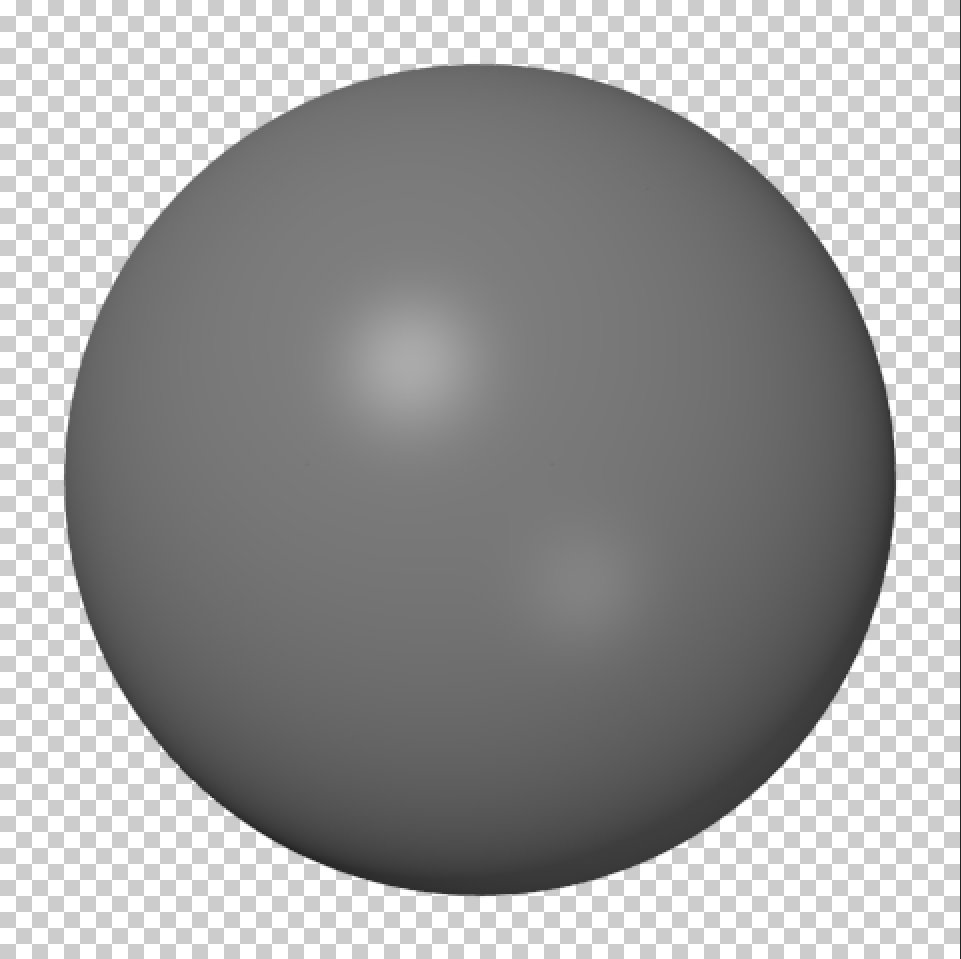
\includegraphics[width=0.7\textwidth, trim=0cm 0cm 0cm 0cm, clip]{visualization/figures/texture_transparent.png}
\end{center}
\caption{The texture used on the billboards is an image of a real sphere rendered with Blender. Notice that the pixels outside the circle are transparent. This allows us to discard these texture pixels in the fragment shader.}
\label{fig:visualization_billboard_texture}
\end{figure}
The fragment shader will then get an interpolated texture coordinate as input, which we will use to look up what RGBA value this pixel gets from the texture. If the alpha value (the opacity) is smaller than one, it means that the pixel contribution comes from a texture pixel outside the circle. In that case we just discard it. We almost forgot one last detail, the \textit{color} of the particles. Again we assume that all particles have the same color (if not, we just use multiple VBO's per timestep), so as we did with the billboard size variable, the color is available as a uniform. The final pixel color is then found by equation \eqref{eq:opengl_combining_colors_textures}
\begin{align}
	\nonumber
	\vec C(\vec p) = \vec c_t[\vec t(\vec p)] \odot \vec c(\vec p).
\end{align}
The fragment shader code is shown in listing \ref{lst:simplefragmentshaderbillboard} with the final rendering result in figure \ref{fig:visualization_billboard_md}. In this rendered image, we also added light effects making atoms that are far away from the camera appear darker. This increases the feeling of depth which clarifies the pores.
\begin{lstlisting}[caption=billboardFragmentShader.glsl, label=lst:simplefragmentshaderbillboard, language=GLSL]
#version 330
uniform vec4 color;
uniform sampler2D qt_Texture0;
in vec2 texCoord;
out vec4 MyFragColor;

void main(void) {
    MyFragColor  = texture2D(qt_Texture0, texCoord.st);
    MyFragColor  = MyFragColor * color;
    if(MyFragColor.a < 0.9999) {
        discard;
    }
}

\end{lstlisting}

\begin{figure}[h]
\begin{center}
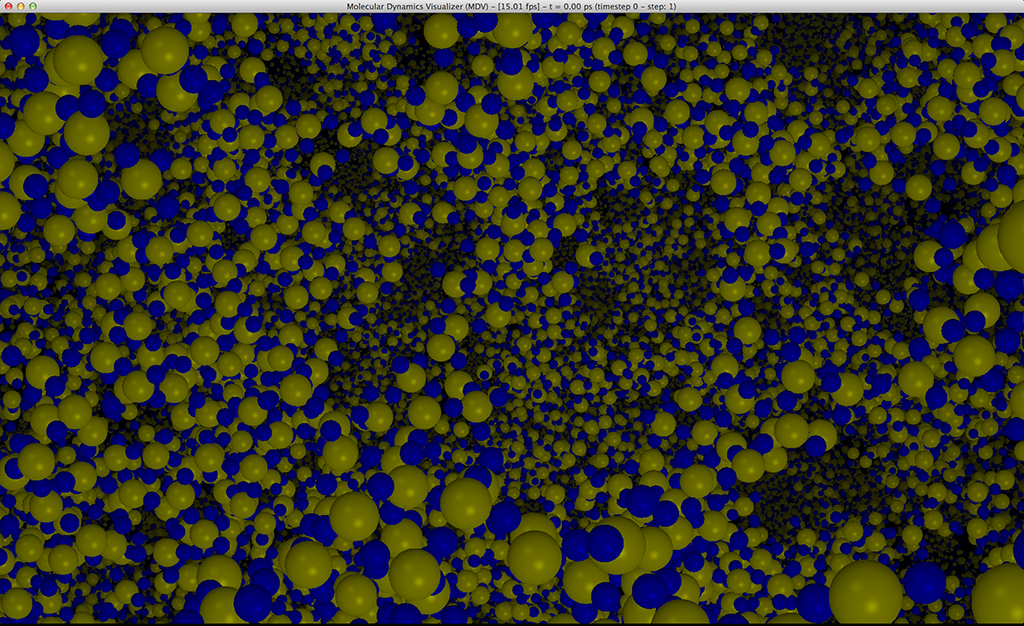
\includegraphics[width=\textwidth, trim=0cm 0cm 0cm 0cm, clip]{visualization/figures/billboards_md_visualization.png}
\end{center}
\caption{The final rendered image with an MD simulation using billboards. In the rendering, light effects are added to increase the feeling of depth, clarifying the pore structure. The atoms form a nanoporous SiO$_2$ system simulated with the REMD22 code developed at USC.}
\label{fig:visualization_billboard_md}
\end{figure}

\subsection{Periodic copies}
We used the geometry shader to create a \textit{GL\_TRIANGLE\_STRIP} creating the billboard from one single vertex (the particle position). Then, one may ask, why not use the geometry shader to create \textit{several} billboards, adding periodic copies of every particle in the system? This makes sense if the simulation operates with periodic boundary conditions so we have periodic symmetry on all directions. So, if the system is a box of size $L_x\times L_y \times L_z$, we can create 26 copies of the whole system giving a larger box of size $3L_x\times 3L_y\times 3L_z$, making the impression that the system is larger. This provides an important effect near the boundaries of the system, see figure \ref{fig:visualization_billboard_periodic_copies}.
\begin{figure}[htb]
\begin{center}
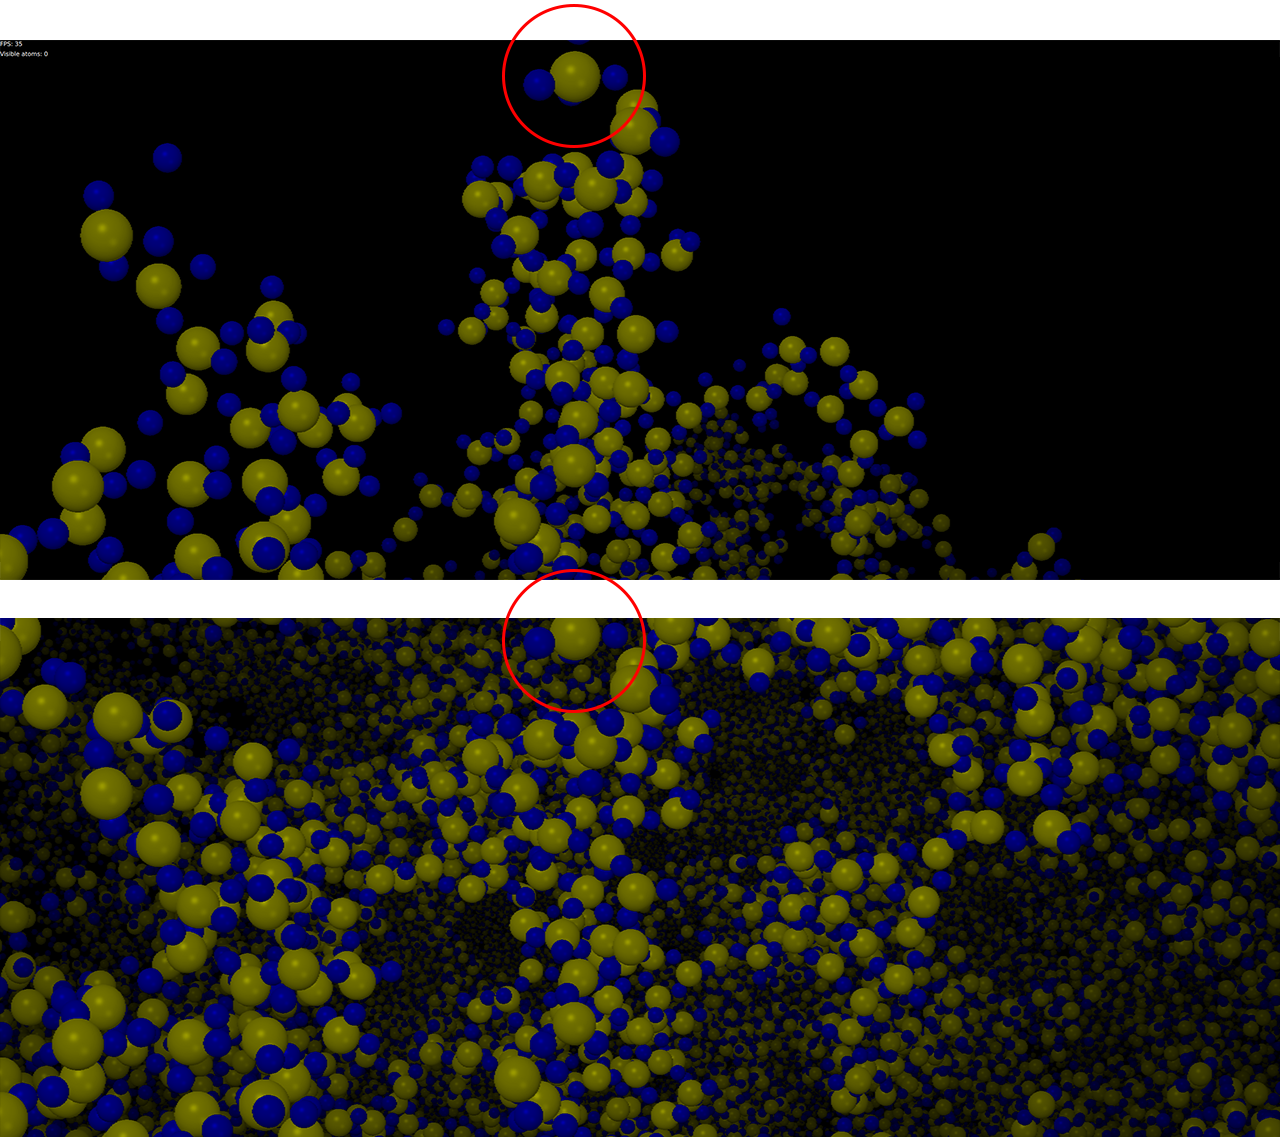
\includegraphics[width=0.9\textwidth, trim=0cm 0cm 0cm 0cm, clip]{visualization/figures/periodic_copies.png}
\end{center}
\caption{Adding periodic copies of the system provides an important effect when looking at atoms near the boundary. The upper image shows a visualization with no periodic copies of the atoms. This shows that the system clearly has a finite size. In the lower image, by adding 26 periodic copies of the whole system, it is not obvious that we are at the edge of the system.}
\label{fig:visualization_billboard_periodic_copies}
\end{figure}
We will use a feature in OpenGL called geometry shader instancing to add all the copies. With instancing, the geometry shader is executed 27 times per input vertex. We can use the variable \textit{gl\_InvocationID} to identify which of the 27 instances we are running. The system coordinate $(S_x, S_y, S_z), S_i \in \{-1, 0, 1\}$ for invocation id $i$ is calculated as
\begin{align}
	S_x =& (i\bmod 3) - 1\\
	S_y =& (\ceil{i/3}\bmod 3) - 1\\
	S_z =& (\ceil{i/9}) - 1,
\end{align}
where $\ceil{a}$ is the ceiling function. One instance of the geometry shader should then render a billboard displaced with 
\begin{align}
	\vec d = (L_x\cdot S_x, L_y\cdot S_y, L_z\cdot S_z),
\end{align}
where the system size $(L_x, L_y, L_z)$ is available as a uniform. The displacement $\vec d$ is given in the model space, so we must transform it the projection space before we add it to the position vertex (which, as we remember, already is in the projection space). The full geometry shader code using instancing to add periodic copies is found in listing \ref{lst:fullgeometryshaderbillboard}.
\begin{lstlisting}[caption=billboardGeometryShaderWithPeriodicCopies.glsl, label=lst:fullgeometryshaderbillboard, language=GLSL]
#version 400
layout(invocations=27) in;
layout(points) in;
layout(triangle_strip, max_vertices = 4) out;
uniform mat4 qt_ProjectionMatrix;
uniform mat4 qt_ModelViewProjectionMatrix;
uniform vec2 size;
uniform vec3 systemSize;
out vec2 texCoord;

void main(void) {
  int x = gl_InvocationID % 3 - 1;
  int y = (gl_InvocationID/3) % 3-1;
  int z = (gl_InvocationID/9)-1;
    
  vec4 displacement = vec4(systemSize.x*x,systemSize.y*y,systemSize.z*z,0);
  vec4 pos = gl_in[0].gl_Position + qt_ModelViewProjectionMatrix * displacement;
  gl_Position = pos + qt_ProjectionMatrix*vec4(-size.x, -size.y, 0.0, 0.0);
  texCoord = vec2(0.0, 0.0);
  EmitVertex();
  gl_Position = pos + qt_ProjectionMatrix*vec4(-size.x, size.y, 0.0, 0.0);
  texCoord = vec2(0.0, 1.0);
  EmitVertex();
  gl_Position = pos + qt_ProjectionMatrix*vec4(size.x, -size.y, 0.0, 0.0);
  texCoord = vec2(1.0, 0.0);
  EmitVertex();
  gl_Position = pos + qt_ProjectionMatrix*vec4(size.x, size.y, 0.0, 0.0);
  texCoord = vec2(1.0, 1.0);
  EmitVertex();
  EndPrimitive();
}
\end{lstlisting}
\subsection{Rendering benchmark}
\label{sec:vis_benchmark}
A typical benchmark for a visualization program is the number of frames per second (FPS) the program is able to render a given amount of primitives. In this benchmark, we have used the multibillboard class\footnote{Source code available from \url{http://github.com/ComputationalPhysics/compphys-qt3d-additions}.} that has implemented the shader pipeline explained above. It renders a box with $N$ billboard spheres and adds 26 copies in the geometry shader making the total number of visible spheres $N_\text{spheres} = 27N$. In table \ref{tab:vis_fps_scaling} we have shown a representable subset of the data showing the performance of the billboard class. We have run the program with the number of visible spheres in the range a few thousand to more than one billion. In figure \ref{fig:rendering_benchmark} we have plotted the data from table \ref{tab:vis_fps_scaling} with more data points near the sudden drops of frame rate. We assume that these drops can be explained by meeting different limits on the graphics card. It seems to happen at specific number of vertices emitted by the geometry shader, so our guess would be the bandwidth on the GPU. We have not used any shader profiling tools, so we cannot draw any conclusion without further investigation. 
\begin{table}[htb]
\begin{center}
    \begin{tabular}{|l|l|}
    \hline
    $N_\text{spheres}$ & FPS\\ \hline
    3,375      & $62.09 \pm 3.236$\\
    \hline
    27,000     & $61.80 \pm 3.149$\\
    \hline
    729,000    & $62.03 \pm 3.088$\\
    \hline
    5,832,000   & $62.28 \pm 3.061$\\
    \hline
    19,034,163  & $30.51 \pm 1.601$\\
    \hline
    27,000,000  & $30.36 \pm 1.436$\\
    \hline
    45,499,293  & $20.81 \pm 2.276$\\
    \hline
    70,957,944  & $15.15 \pm 0.879$\\
    \hline
    110,592,000 & $12.14 \pm 2.180$\\
    \hline
    132,651,000 & $9.99 \pm 1.066$\\
    \hline
    287,496,000 & $4.78 \pm 0.8532$\\
    \hline
    421,875,000 & $3.29 \pm 0.4548$\\
    \hline
    1,061,208,000 & $1.40 \pm 0.2386$\\
    \hline
    \end{tabular}
    \caption{Benchmark showing the number of frames per second (FPS) the billboard class is able to render with the number of billboard spheres from a few thousand to more than one billion visible spheres. The benchmark is performed on an NVIDIA GTX Titan.}
    \label{tab:vis_fps_scaling}
    \end{center}
\end{table}

\begin{figure}[htb]
\begin{center}
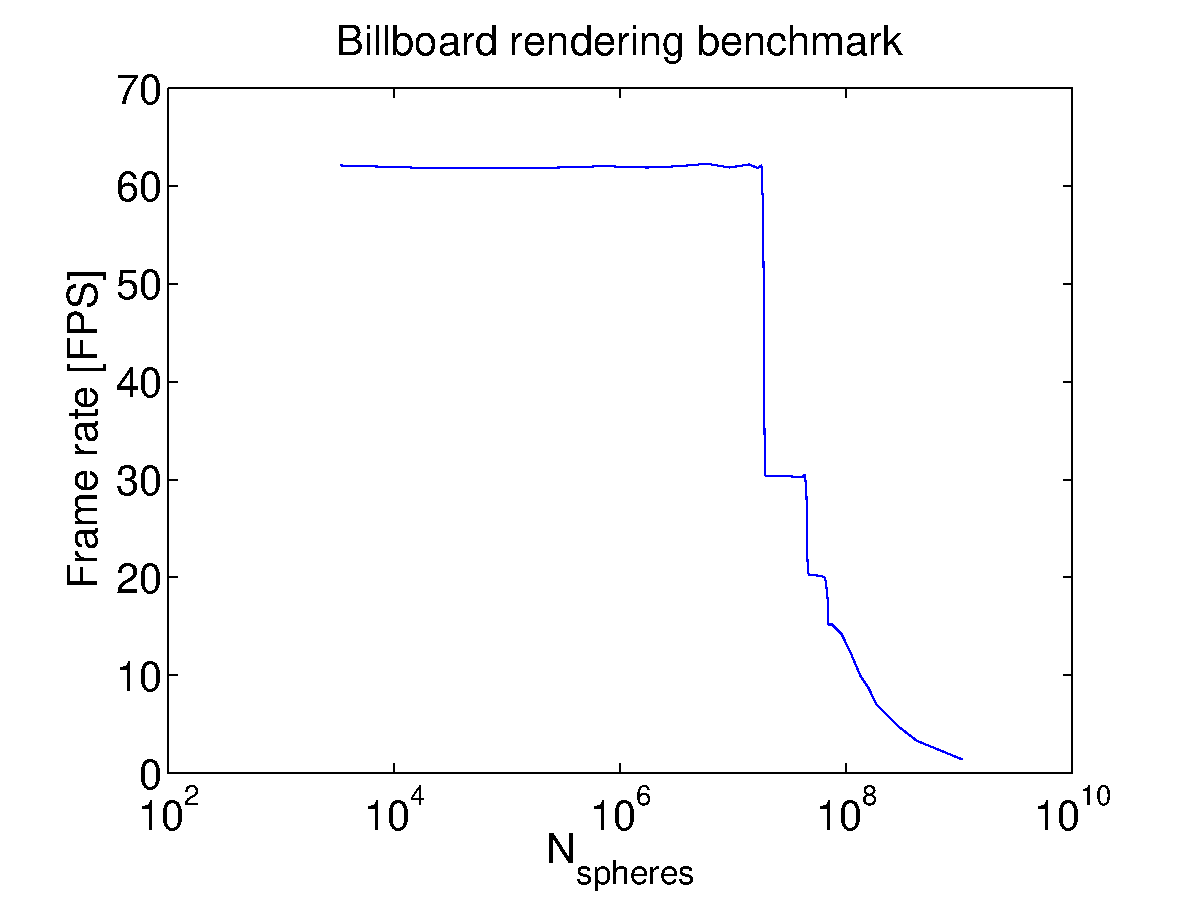
\includegraphics[width=0.8\textwidth, trim=0cm 0cm 0cm 0cm, clip]{visualization/figures/benchmark.eps}
\end{center}
\caption{Benchmark showing the number of frames per second (FPS) the billboard class is able to render with the number of billboard spheres from a few thousand to more than one billion visible spheres. The benchmark is performed on an NVIDIA GTX Titan. The sudden drops in FPS at specific number of spheres are probably explained by reaching the bandwidth limit in the different shader stages.}
\label{fig:rendering_benchmark}
\end{figure}
The visualization tool for an MD state does not need anything else than what we now have presented. The timesteps containing the positions of all the atoms are uploaded to the graphics card as VBOs and the atoms are rendered as points into the rendering pipeline where the billboards are created in the geometry shader. This same rendering technique can of course be used to render the particles in a DSMC simulation, but we want to render the complex geometry that the particles interact with. We will use what's called marching cubes for this.